% GDS-ParT-MoE -- Technical report: architecture, mathematics and first results
% Build (from docs/): pdflatex GDS-ParT-MoE_Technical_Report.tex   (run twice for the table of contents)
\documentclass[11pt,a4paper]{article}

\usepackage[margin=2.3cm]{geometry}
\usepackage[T1]{fontenc}
\usepackage[utf8]{inputenc}
\usepackage{lmodern}
\usepackage{amsmath,amssymb}
\usepackage{booktabs}
\usepackage{tabularx}
\usepackage{graphicx}
\usepackage{xcolor}
\usepackage{enumitem}
\usepackage{listings}
\usepackage{tikz}
\usetikzlibrary{arrows.meta,positioning,fit,backgrounds,calc}
\usepackage[colorlinks=true,linkcolor=blue!50!black,urlcolor=blue!50!black]{hyperref}

\definecolor{accent}{HTML}{2E86AB}
\lstset{basicstyle=\ttfamily\small,columns=fullflexible,frame=single,framerule=0.3pt,
        breaklines=true,keepspaces=true,showstringspaces=false}
\newcommand{\code}[1]{\texttt{\detokenize{#1}}}
\newcommand{\R}{\mathbb R}
\newcommand{\softmax}{\operatorname{softmax}}
\newcommand{\LN}{\operatorname{LN}}
\newcommand{\GELU}{\operatorname{GELU}}
\newcommand{\FFN}{\operatorname{FFN}}
\newcommand{\Drop}{\operatorname{Drop}}
\newcommand{\MLP}{\operatorname{MLP}}
\newcommand{\TopK}{\operatorname{TopK}}
\newcommand{\NMI}{\operatorname{NMI}}
\newcommand{\Had}{\odot}
\setlist{itemsep=2pt,topsep=4pt}
\setlength{\emergencystretch}{3em}
\sloppy

\title{\textbf{GDS-ParT-MoE}\\[4pt]\large A per-particle mixture of experts for the Gated
Dual-Stream Particle Transformer\\[2pt]
\normalsize Architecture, mathematics, training and first expert-specialisation results}
\author{Avinash Chandra Gupta\\\small \url{https://github.com/Avinashistoocool/GDS-parT-MoE}}
\date{Version 1.0.0 \quad October 2026}

\hypersetup{pdfauthor={Avinash Chandra Gupta},pdfkeywords={Avinash Chandra Gupta, Avinash Gupta}}
\begin{document}
\maketitle

\begin{abstract}
GDS-ParT-MoE replaces the particle-level feed-forward networks of the Gated Dual-Stream
Particle Transformer (GDS-ParT) with a token-choice mixture of experts. Each real jet
constituent is routed to the top $k=2$ of $E=8$ expert FFNs, and only padding is excluded.
Because the router sees one particle at a time, its decisions can be compared directly with
that particle's physics: species, charge, momentum share, angle to the jet axis, transverse
impact parameter, and the Lund-plane variables of its nearest neighbour. The model is built
by sparse upcycling from a trained dense GDS-ParT checkpoint, which makes the untrained MoE
reproduce the dense network exactly. This report documents the motivation, the architecture,
every equation used by the code (router, renormalised top-$k$ mixture, Switch-style
load-balancing loss, router $z$-loss, upcycling, optimisation schedule and evaluation
metrics), and the expert-analysis toolkit (routing statistics, physics profiles, normalised
mutual information and expert knockout). It closes with the first, preliminary result: after a
single fine-tuning epoch on 300k JetClass jets the 8-expert model reaches validation accuracy
0.8472 (dense: 0.8487), and its first-layer router already partitions particles by charge and
species (normalised mutual information 0.45 and 0.43), while deeper layers remain close to
uniform.
\end{abstract}

\tableofcontents
\newpage

%====================================================================
\section{Motivation}
%====================================================================

Jet-tagging transformers such as ParT and GDS-ParT classify a jet from its constituents with
high accuracy, but it is hard to say \emph{what} a given layer has learned. Attention maps
are one handle, yet they describe pairs, depend on the value vectors and later layers, and
are difficult to relate to a single physical property.

A mixture of experts (MoE) offers a different handle. If the feed-forward part of each block
is split into several experts and a router decides, for every particle separately, which
experts process it, then the routing decision is a discrete, per-particle label that the
network itself chose. One can then ask simple questions:

\begin{itemize}
  \item Does an expert handle one particle species (photons, neutral hadrons, leptons)?
  \item Does it handle the hard core of the jet, or soft wide-angle radiation?
  \item Does it handle displaced tracks, as produced by $b$ and $c$ hadron decays?
  \item Does it handle collinear splittings, i.e.\ a particular region of the Lund plane?
  \item Which jet classes rely on it, in the sense that removing it hurts their accuracy?
\end{itemize}

If the experts specialise, the routing table is a learned partition of particle phase
space. If they do not, the router entropy and the mutual-information numbers say so
directly. The project was carried out under the supervision of Prof.\ Abhishek Iyer between
May and July 2026.

The design goal was to change as little as possible of GDS-ParT. Attention, the relational
query/key gates, the additive pairwise bias, the class-attention (CLS) blocks and the
classifier are the original modules from \code{gds_part_colab.py}. Only the particle FFNs
become MoE layers.

%====================================================================
\section{Background: the dense GDS-ParT block}
%====================================================================

The notation follows the GDS-ParT mathematical notes. A jet has $N$ constituent slots with
padding mask $m_i\in\{0,1\}$ (1 for a real particle). Each particle carries 17 normalised
features $f_i\in\R^{17}$, and each pair carries the four ParT interaction features
\begin{equation}
 U_{ij}=(\ln\Delta_{ij},\ \ln k_{T,ij},\ \ln z_{ij},\ \ln m_{ij}^2),
\end{equation}
computed on the GPU from the constituent four-vectors (\code{data/jetclass_cache.py}).

The model width is $D=128$ with $H=8$ heads, $L=8$ particle blocks, FFN hidden width
$D_{\rm ff}=512$, pair-embedding width $D_p=64$, dropout $0.1$ and at most 128 particles.
Particle and pair embeddings are
\begin{align}
 x_i^{(0)}&=\Drop\big(W_2\GELU(W_1\LN(f_i)+b_1)+b_2\big)\in\R^{D},\\
 r_{ij}&=W_4\GELU(W_3U_{ij}+b_3)+b_4\in\R^{D_p}.
\end{align}
In the checkpoint used here (\code{v2_shared}) the relational gate is shared by all blocks
and uses a masked mean over neighbours,
\begin{equation}
 s_i=\frac{\sum_j m_j r_{ij}}{\max(1,\sum_j m_j)},\qquad
 g_i^{a}=1+\tanh\!\big(\MLP_a(s_i)\big),\quad a\in\{Q,K\},
\end{equation}
with the last layer of each gate MLP zero-initialised so that $g=1$ at initialisation. A
per-head additive pair bias $\mathcal B_{ij}^{(h)}=W_{\rm bias}r_{ij}+b_{\rm bias}$ is shared by
all blocks. One dense pre-LN block $\ell$ computes
\begin{align}
 h_i&=\LN_1(x_i),\\
 q'_i&=(W_Qh_i+b_Q)\Had g_i^Q,\qquad k'_i=(W_Kh_i+b_K)\Had g_i^K,\qquad v_i=W_Vh_i+b_V,\\
 A^{(h)}_{ij}&=\softmax_j\!\Big(q_i'^{(h)\top}k_j'^{(h)}/\sqrt{d}+\mathcal B^{(h)}_{ij}
   +\log m_j\Big),\qquad d=D/H=16,\\
 \tilde x_i&=x_i+W_O\operatorname{concat}_h\Big(\sum_jA^{(h)}_{ij}v_j^{(h)}\Big)+b_O,\\
 x_i^{\rm next}&=\tilde x_i+\FFN(\LN_2(\tilde x_i)),
 \label{eq:dense-ffn}
\end{align}
where $\log m_j$ is $0$ for real particles and $-\infty$ for padding, and
\begin{equation}
 \FFN(u)=\Drop\big(W^{\rm out}\,\Drop(\GELU(W^{\rm in}u+b^{\rm in}))+b^{\rm out}\big),
 \qquad W^{\rm in}\in\R^{512\times128},\ W^{\rm out}\in\R^{128\times512}.
\end{equation}
After the eight particle blocks, two class-attention blocks update a learned CLS token, and
a two-layer classifier maps $\LN(c)$ to ten logits. The MoE extension touches only
equation~\eqref{eq:dense-ffn}.

%====================================================================
\section{Architecture}
%====================================================================

\begin{figure}[t]
\centering
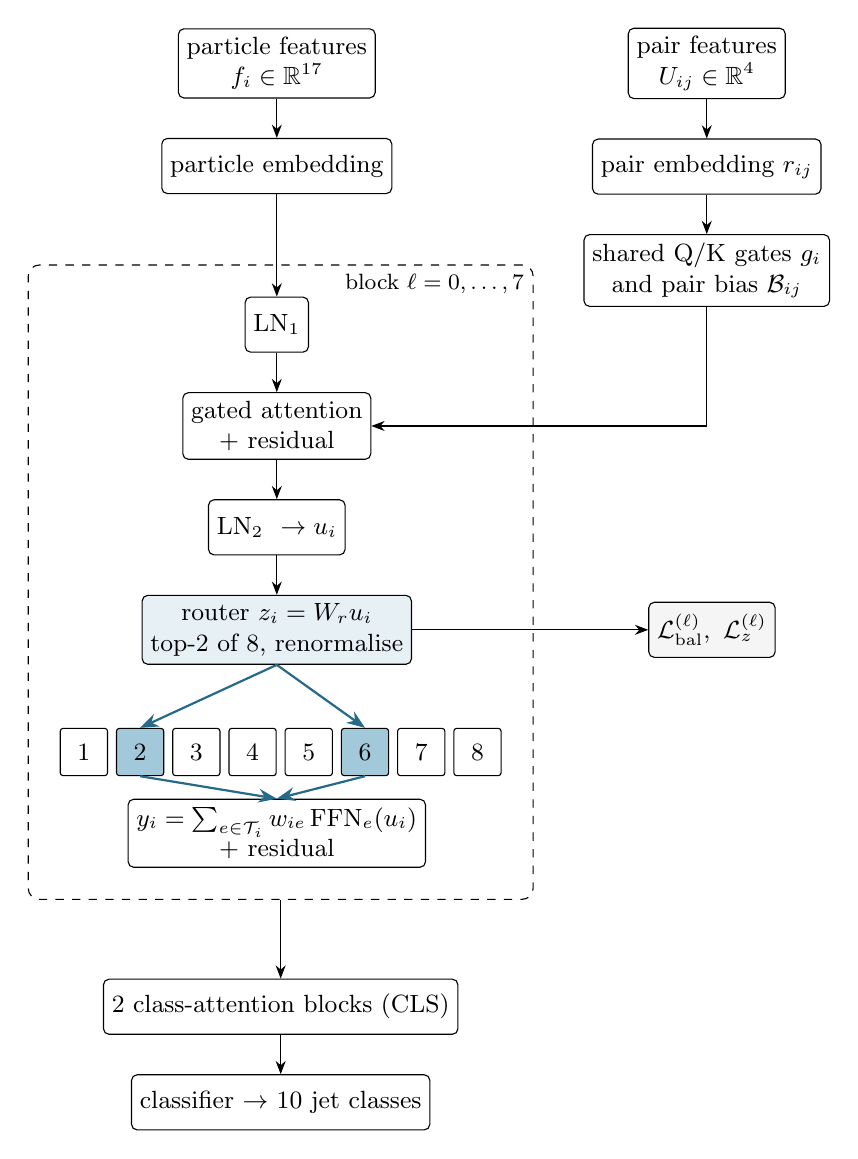
\begin{tikzpicture}[
  font=\small, >=Stealth,
  box/.style={draw, rounded corners=2pt, align=center, minimum height=7mm, inner sep=3pt, fill=white},
  moe/.style={box, fill=accent!12},
  exp/.style={draw, rounded corners=1pt, minimum width=6mm, minimum height=6mm, inner sep=1pt, fill=white},
  sel/.style={exp, fill=accent!45},
  node distance=5mm and 7mm]
 \node[box] (pf) {particle features\\$f_i\in\R^{17}$};
 \node[box, below=of pf] (pe) {particle embedding};
 \node[box, right=32mm of pf] (uf) {pair features\\$U_{ij}\in\R^{4}$};
 \node[box, below=of uf] (ue) {pair embedding $r_{ij}$};
 \node[box, below=of ue] (gate) {shared Q/K gates $g_i$\\and pair bias $\mathcal B_{ij}$};

 \node[box, below=13mm of pe] (ln1) {$\LN_1$};
 \node[box, below=of ln1] (att) {gated attention\\$+$ residual};
 \node[box, below=of att] (ln2) {$\LN_2$ \ $\to u_i$};
 \node[moe, below=of ln2] (router) {router $z_i=W_ru_i$\\top-2 of 8, renormalise};
 \node[exp, below=8mm of router, xshift=-24.5mm] (e0) {$1$};
 \node[sel, right=1mm of e0] (e1) {$2$};
 \node[exp, right=1mm of e1] (e2) {$3$};
 \node[exp, right=1mm of e2] (e3) {$4$};
 \node[exp, right=1mm of e3] (e4) {$5$};
 \node[sel, right=1mm of e4] (e5) {$6$};
 \node[exp, right=1mm of e5] (e6) {$7$};
 \node[exp, right=1mm of e6] (e7) {$8$};
 \node[box, below=9mm of router, yshift=-8mm] (mix) {$y_i=\sum_{e\in\mathcal T_i}w_{ie}\FFN_e(u_i)$\\$+$ residual};
 \begin{scope}[on background layer]
  \node[draw, dashed, rounded corners, fit=(ln1)(att)(ln2)(router)(e0)(e7)(mix), inner sep=4mm,
        label={[anchor=north east]north east:{\footnotesize block $\ell=0,\dots,7$}}] (blk) {};
 \end{scope}
 \node[box, below=10mm of blk.south] (cls) {2 class-attention blocks (CLS)};
 \node[box, below=of cls] (clf) {classifier $\to$ 10 jet classes};
 \node[box, right=8mm of router, xshift=22mm, fill=gray!8] (aux) {$\mathcal L_{\rm bal}^{(\ell)},\ \mathcal L_z^{(\ell)}$};

 \draw[->] (pf) -- (pe);
 \draw[->] (uf) -- (ue);
 \draw[->] (ue) -- (gate);
 \draw[->] (pe) -- (ln1);
 \draw[->] (ln1) -- (att);
 \draw[->] (gate.south) |- (att.east);
 \draw[->] (att) -- (ln2);
 \draw[->] (ln2) -- (router);
 \foreach \e in {e1,e5} \draw[->, accent!80!black, thick] (router.south) -- (\e.north);
 \foreach \e in {e1,e5} \draw[->, accent!80!black, thick] (\e.south) -- (mix.north);
 \draw[->] (router.east) -- (aux.west);
 \draw[->] (blk.south) -- (cls);
 \draw[->] (cls) -- (clf);
\end{tikzpicture}
\caption{GDS-ParT-MoE. Inside every particle block the FFN is replaced by a router and eight
expert FFNs. Each real particle $i$ is sent to its two highest-probability experts (shaded),
whose outputs are mixed with renormalised weights. Attention, gates, pair bias and CLS
pooling are the unchanged GDS-ParT modules. Each MoE layer also returns a load-balancing and
a $z$-loss term.}
\label{fig:arch}
\end{figure}

Figure~\ref{fig:arch} shows the model. The code lives in \code{moe.py}:

\begin{description}[style=nextline,leftmargin=0pt]
  \item[\code{GDSParTMoEConfig}] extends \code{GDSParTConfig} with \code{n_experts} ($E$,
  default 8), \code{top_k} ($k$, default 2), \code{moe_layers} (indices of blocks that get an
  MoE; default all eight), \code{aux_weight} ($\lambda_{\rm bal}=10^{-2}$) and \code{z_weight}
  ($\lambda_z=10^{-3}$).
  \item[\code{MoEFFN}] the router and the expert list. Each expert is the same
  \code{_ffn(cfg)} module as the dense FFN ($128\to512\to128$ with GELU and dropout).
  \item[\code{GDSParTMoEBlock}] the dense block with \code{self.ffn} replaced by
  \code{MoEFFN} if the block index is in \code{moe_layers}. It returns the new state and a
  two-vector of auxiliary losses (zero for non-MoE blocks).
  \item[\code{GDSParTMoE}] the dense model with these blocks. It sums the auxiliary losses
  of all blocks, stores the weighted sum in \code{self.aux_loss}, and adds helpers for
  recording routing (\code{set_record}) and knocking out experts (\code{disable_experts}).
  \item[\code{upcycle_state_dict}] converts a dense checkpoint into MoE weights
  (Section~\ref{sec:upcycle}).
\end{description}

\subsection{Token selection}
Only real particles are routed. The layer gathers the $T=\sum_{b,i}m_{bi}$ real tokens of the
micro-batch into a matrix $u\in\R^{T\times D}$ (\code{x[mask]}), routes them, and scatters the
outputs back. Padding slots receive an exact zero FFN output and never enter the loss
statistics. Without a mask, all $B N$ slots are treated as real.

\subsection{Router}
For a token $u_i=\LN_2(\tilde x_i)\in\R^{D}$ the router is a bias-free linear map
\begin{equation}
 z_i=W_r u_i\in\R^{E},\qquad W_r\in\R^{E\times D},\qquad (W_r)_{ej}\sim\mathcal N(0,0.02^2)
 \ \text{at initialisation}.
\end{equation}
The logits are cast to float32 even under mixed precision. Disabled experts (knockout,
Section~\ref{sec:knockout}) get $z_{ie}=-\infty$. Routing probabilities are
\begin{equation}
 \pi_{ie}=\frac{\exp z_{ie}}{\sum_{a=1}^{E}\exp z_{ia}}.
\end{equation}

\subsection{Top-$k$ selection and renormalised mixture}
Let $\mathcal T_i=\TopK(\pi_i,k)$ be the indices of the $k$ largest probabilities. The mixing
weights are the selected probabilities renormalised to sum to one,
\begin{equation}
 w_{ie}=\frac{\pi_{ie}}{\max\big(10^{-9},\ \sum_{a\in\mathcal T_i}\pi_{ia}\big)},
 \qquad e\in\mathcal T_i,
\end{equation}
and the MoE output is
\begin{equation}
 y_i=\sum_{e\in\mathcal T_i}w_{ie}\,\FFN_e(u_i),\qquad
 x_i^{\rm next}=\tilde x_i+y_i.
\end{equation}
In code the experts are visited one at a time; expert $e$ processes only the rows routed to
it and its weighted output is accumulated with \code{index_add_}. There is no capacity limit
and no token dropping: every real particle is processed by exactly $k$ experts, however
unbalanced the routing is. The cost of an imbalanced router is therefore compute and
specialisation, never lost tokens.

\paragraph{Why $k=2$ by default.}
With $k\ge2$ the task loss reaches the router through the weights, for example with
$\mathcal T_i=\{a,b\}$,
\begin{equation}
 w_{ia}=\frac{\pi_{ia}}{\pi_{ia}+\pi_{ib}}=\sigma(z_{ia}-z_{ib}),\qquad
 \frac{\partial y_i}{\partial z_{ia}}=w_{ia}w_{ib}\big(\FFN_a(u_i)-\FFN_b(u_i)\big).
\end{equation}
With $k=1$ the single weight is identically one, so the task loss gives the router no gradient
away from selection boundaries; only the auxiliary losses train it. The \code{--top_k 1}
option is still useful for reading routing, but it is not a free improvement.

\subsection{Parameter count}
The $D\to D_{\rm ff}\to D$ expert has $128\cdot512+512+512\cdot128+128=131{,}712$ parameters
and each router has $8\cdot128=1{,}024$. With all eight blocks converted, the MoE adds
$8\,(7\cdot131{,}712+1{,}024)=7{,}384{,}064$ parameters to the dense model's $2{,}074{,}420$,
for $9{,}458{,}484$ in total (this matches \code{n_params} in the training history).
Counting only two experts per layer, roughly $3{,}136{,}308$ parameters act on a given
particle. This is a per-token figure; a batch generally touches all experts.

%====================================================================
\section{Auxiliary losses}
%====================================================================

Let $T$ be the number of real tokens in the micro-batch, $\mathbb 1[\cdot]$ the indicator and
$\mathcal A\subseteq\{1,\dots,E\}$ the set of live (not knocked out) experts, $E_{\rm live}=|\mathcal A|$.
During training $\mathcal A$ is all experts and $E_{\rm live}=E=8$.

\subsection{Switch load-balancing loss}
The dispatch fraction and the mean router probability of expert $e$ are
\begin{equation}
 f_e=\frac{1}{Tk}\sum_{i=1}^{T}\mathbb 1[e\in\mathcal T_i],\qquad
 \bar\pi_e=\frac1T\sum_{i=1}^{T}\pi_{ie},
\end{equation}
and the balance loss is
\begin{equation}
 \mathcal L_{\rm bal}=E_{\rm live}\sum_{e\in\mathcal A}f_e\,\bar\pi_e .
\end{equation}
Both $f$ and $\bar\pi$ sum to one. For a perfectly uniform router $f_e=\bar\pi_e=1/E$ and
$\mathcal L_{\rm bal}=1$; concentrating load on a few experts raises it. The indicator is not
differentiable, so the gradient flows through $\bar\pi_e$: experts that already receive many
tokens get their probabilities pushed down.

\subsection{Router $z$-loss}
\begin{equation}
 \mathcal L_z=\frac1T\sum_{i=1}^{T}\Big(\log\sum_{e=1}^{E}\exp\tilde z_{ie}\Big)^2,
 \qquad \tilde z_{ie}=\begin{cases}z_{ie}&e\in\mathcal A\\0&e\notin\mathcal A\end{cases}.
\end{equation}
It keeps the router logits small, which keeps the softmax away from saturation and helps
numerical stability under float16 autocast. (Replacing knocked-out logits by zero only avoids
an infinite value during analysis; it does not affect training.)

\subsection{Total objective}
Each block returns $(\mathcal L_{\rm bal}^{(\ell)},\mathcal L_z^{(\ell)})$, zero for non-MoE
blocks. The model stores
\begin{equation}
 \mathcal L_{\rm aux}=\lambda_{\rm bal}\sum_{\ell}\mathcal L_{\rm bal}^{(\ell)}
   +\lambda_z\sum_{\ell}\mathcal L_z^{(\ell)},\qquad
 \lambda_{\rm bal}=10^{-2},\ \lambda_z=10^{-3},
\end{equation}
summed (not averaged) over layers, and the training loss for a micro-batch is
\begin{equation}
 \mathcal L=\mathrm{CE}_{\varepsilon}(\ell,y)+\mathcal L_{\rm aux},\qquad
 \mathrm{CE}_\varepsilon=-(1-\varepsilon)\log p_y-\frac{\varepsilon}{C}\sum_{c=1}^{C}\log p_c,
\end{equation}
with label smoothing $\varepsilon=0.1$ and $C=10$ classes. With eight uniform MoE layers the
balance term contributes about $8\times10^{-2}\times1=0.08$ to the loss. Lowering
\code{--aux_weight} trades balance for sharper specialisation.

%====================================================================
\section{Sparse upcycling}
\label{sec:upcycle}
%====================================================================

Training an MoE from scratch on JetClass is expensive. Instead, \code{--init_dense} loads a
trained dense GDS-ParT checkpoint and copies it into the MoE (\code{upcycle_state_dict}):

\begin{enumerate}
 \item Every non-FFN tensor (embeddings, gates, attention, pair bias, CLS blocks, classifier)
   is copied unchanged.
 \item For each MoE block $\ell$, every expert receives a copy of that block's dense FFN
   weights. With \code{--upcycle_noise} $\sigma$ (default $0.01$), each weight matrix (tensors
   with more than one dimension) is perturbed,
   \begin{equation}
    W^{(e)}=W+\sigma\,\operatorname{std}(W)\,\xi^{(e)},\qquad \xi^{(e)}_{ab}\sim\mathcal N(0,1),
   \end{equation}
   while biases are copied exactly. The noise breaks the symmetry between experts so that
   they can diverge.
 \item Routers keep their fresh $\mathcal N(0,0.02^2)$ initialisation.
\end{enumerate}

\paragraph{Exact equivalence for $\sigma=0$.}
If every expert equals the dense FFN $f$, then for any router and any top-$k$ set
\begin{equation}
 y_i=\sum_{e\in\mathcal T_i}w_{ie}f(u_i)=f(u_i)\sum_{e\in\mathcal T_i}w_{ie}=f(u_i),
\end{equation}
because the renormalised weights sum to one. The untrained MoE therefore reproduces the
dense model in evaluation mode, up to floating-point rounding. The unit test
\code{test_upcycle_matches_dense} checks this to $10^{-5}$ on random inputs after perturbing
all dense parameters (so that the identity-initialised gates are not trivially one). With
$\sigma=0.01$ the equivalence is approximate; README reports validation accuracy 0.8479 for
the upcycled model before fine-tuning against 0.8487 for the dense checkpoint.

%====================================================================
\section{Training}
%====================================================================

\code{train_moe.py} trains on the memory-mapped JetClass cache built by the GDS-ParT
trainer. The cache stores float16 particle features and float32 four-vectors in ragged form;
batches are padded only to their longest jet, and training batches are formed from pools of
jets bucketed by multiplicity to reduce the $O(N^2)$ pair cost. The pair features $U_{ij}$
are computed on the GPU per batch.

\begin{table}[ht]
\centering
\small
\begin{tabularx}{\linewidth}{@{}>{\raggedright\arraybackslash}p{0.28\linewidth}>{\raggedright\arraybackslash}X>{\raggedright\arraybackslash}p{0.26\linewidth}@{}}
\toprule
Setting & Flag & Default\\
\midrule
Experts / top-$k$ / MoE blocks & \code{--n_experts}, \code{--top_k}, \code{--moe_layers} & 8 / 2 / all\\
Balance and $z$ weights & \code{--aux_weight}, \code{--z_weight} & $10^{-2}$, $10^{-3}$\\
Upcycling noise & \code{--upcycle_noise} & 0.01\\
Optimiser & AdamW & lr $2\times10^{-4}$, weight decay $10^{-2}$\\
Router learning-rate multiplier & \code{--router_lr_mult} & 5 (router lr $10^{-3}$)\\
Warm-up / schedule & \code{--warmup_frac} & 3\,\% linear, then cosine to 0\\
Gradient clipping & \code{--grad_clip} & global norm 1.0\\
Label smoothing & \code{--label_smoothing} & 0.1\\
Batch size & \code{--batch_size} & 512 jets\\
Pair budget per micro-batch & \code{--max_pairs_per_step} & $2\times10^{6}$\\
Precision & \code{--amp} & float16 autocast with GradScaler\\
Epochs & \code{--epochs} & 3\\
\bottomrule
\end{tabularx}
\caption{Training settings in \code{train_moe.py}.}
\label{tab:train}
\end{table}

\paragraph{Optimiser.} The parameters are split into two AdamW groups: router weights (any
name containing \code{.router.}) with learning rate $5\eta$, and everything else with
$\eta=2\times10^{-4}$. The routers are new, while the rest of the network is already trained,
so the routers are allowed to move faster.

\paragraph{Schedule.} With $S$ total optimiser steps and $S_w=\lfloor0.03S\rfloor$ warm-up
steps, the learning-rate multiplier at step $s$ is
\begin{equation}
 \rho(s)=\begin{cases}
 s/\max(1,S_w) & s<S_w,\\[2pt]
 \tfrac12\Big(1+\cos\big(\pi\min\big(1,\tfrac{s-S_w}{\max(1,S-S_w)}\big)\big)\Big) & s\ge S_w.
 \end{cases}
\end{equation}

\paragraph{Micro-batching.} A batch of $B$ jets padded to $N$ particles is split into
micro-batches of $\max(1,\min(B,\lfloor 2\times10^6/N^2\rfloor))$ jets so that the
$B\times N\times N$ pair tensors fit in memory. Each micro-batch loss is scaled by its share
$b/B$ of the batch before the backward pass, so the accumulated gradient is that of the
batch-mean loss. The auxiliary losses are computed per micro-batch, i.e.\ $f_e$ and
$\bar\pi_e$ are micro-batch statistics. In training mode each block is also wrapped in
activation checkpointing.

\paragraph{Evaluation and checkpoints.} After each epoch the model is evaluated on the
validation cache (at most \code{--val_max_jets}, default 100{,}000, drawn with a fixed seed)
and \code{best.pt} and \code{last.pt} are written together with \code{history.json}.

%====================================================================
\section{Metrics}
%====================================================================

\code{metrics.py} follows the definitions of the ParT paper. For softmax scores
$p\in\R^{n\times C}$ and labels $y$:
\begin{itemize}
 \item \textbf{Accuracy}: $\frac1n\sum_j\mathbb 1[\arg\max_c p_{jc}=y_j]$.
 \item \textbf{Macro one-vs-one AUC}: the scikit-learn \code{roc_auc_score} with
   \code{average="macro"}, \code{multi_class="ovo"}.
 \item \textbf{Background rejection}: for each signal class $S$ against QCD, restrict to
   jets of those two classes and use the two-class score
   \begin{equation}
    t_j=\frac{p_{jS}}{p_{jS}+p_{j,\rm QCD}+10^{-12}}.
   \end{equation}
   The false-positive rate at a target signal efficiency (true-positive rate) $\epsilon_S$ is
   read off the ROC curve by linear interpolation, and $\mathrm{Rej}_{\epsilon_S}=1/\mathrm{FPR}$.
   The targets are $\epsilon_S=50\,\%$ for Hbb, Hcc, Hgg, H4q, Tbqq, Wqq and Zqq,
   $99\,\%$ for Hqql and $99.5\,\%$ for Tbl.
 \item \textbf{Per-class accuracy}: $\Pr(\arg\max p=c\mid y=c)$, also used by the knockout study.
\end{itemize}

%====================================================================
\section{Expert analysis}
%====================================================================

\code{analyze_experts.py} loads a checkpoint, runs it in evaluation mode on validation jets
with routing recording switched on, and relates the routing of every real particle in every
MoE layer to physics quantities.

\subsection{Recorded routing}
For particle $i$ in MoE layer $\ell$ the script keeps the full probability vector
$\pi^{(\ell)}_i$ and the top-1 expert $t^{(\ell)}_i=\arg\max_e\pi^{(\ell)}_{ie}$ (the first of
the top-$k$ indices). All statistics below use $t^{(\ell)}_i$.

\subsection{Physics variables}
The cached features are normalised, so the script inverts the normalisation:
\begin{align}
 \text{type}_i&=\arg\max(f_{i,8},\dots,f_{i,12})\in\{\text{ch.\ had},\text{neu.\ had},\gamma,e,\mu\},\\
 q_i&=\operatorname{round}(f_{i,7}),
 &\ln p_{T,i}&=f_{i,0}/0.7+1.7,\\
 z_i&=p_{T,i}/p_{T,\rm jet}=\exp(f_{i,2}/0.7-4.7),
 &\Delta R_i&=f_{i,4}/4+0.2,\\
 |\tanh d_0|_i&=|f_{i,13}|.
\end{align}
These are exact inverses only inside the $[-5,5]$ clipping range of the cache and up to
float16 rounding. From the four-vectors it also computes, with rapidity $y$ and wrapped
azimuth difference,
\begin{align}
 \Delta_{ij}&=\sqrt{(y_i-y_j)^2+\delta\phi_{ij}^2},\qquad
 j^\ast(i)=\arg\min_{j\ne i,\ m_j=1}\Delta_{ij},\\
 \Delta R^{\rm nn}_i&=\Delta_{i j^\ast},\qquad
 \ln k_{T,i}^{\rm nn}=\ln\max\big(10^{-4},\ \min(p_{T,i},p_{T,j^\ast})\,\Delta R^{\rm nn}_i\big),
\end{align}
the nearest-neighbour distance and the Lund-plane $k_T$ of that closest pair, and the
$p_T$ rank of the particle inside its jet (0 for the hardest). Each particle also carries
its jet's truth class and multiplicity.

\subsection{Routing statistics}
For each layer, with $n$ recorded particles:
\begin{align}
 \text{load}_e&=\frac1n\sum_i\mathbb 1[t_i=e],\\
 \bar H&=\frac1n\sum_i\Big(-\sum_e\pi_{ie}\ln(\pi_{ie}+10^{-9})\Big),\qquad
 \bar H\le\ln E=\ln 8\approx2.08\ \text{nats},\\
 P(e\mid\text{type}=\tau)&=\frac{\sum_i\mathbb 1[t_i=e,\ \text{type}_i=\tau]}{\sum_i\mathbb 1[\text{type}_i=\tau]},
 \qquad P(e\mid\text{class}=c)\ \text{analogously},\\
 \text{enrich}_{e,\tau}&=P(e\mid\tau)/\text{load}_e .
\end{align}
The per-expert \emph{physics profile} is the mean of each variable over the particles whose
top-1 expert is $e$, plus the charged fraction $\Pr(q\ne0\mid t=e)$. The plain-language report
flags a variable as high or low for an expert when its profile value is more than one
standard deviation (across the eight experts) above or below the expert average.

\subsection{Normalised mutual information}
For the expert label $t$ and a discrete variable $v$,
\begin{equation}
 \NMI(t;v)=\frac{I(t;v)}{\min\big(H(t),H(v)\big)},\qquad
 I(t;v)=\sum_{a,b}p(a,b)\ln\frac{p(a,b)}{p(a)p(b)},
\end{equation}
computed from the empirical joint histogram. Particle type, charge (shifted to
$\{0,1,2\}$) and jet class are used directly; each continuous variable is cut into ten
quantile bins (deciles, merged where edges coincide). $\NMI=0$ means the routing carries no
information about $v$; $\NMI=1$ means one determines the other up to the smaller entropy.

\subsection{Expert knockout}
\label{sec:knockout}
\code{disable_experts} sets the logits of chosen experts to $-\infty$. The softmax then
renormalises over the live experts and the top-$k$ is taken among them, so each affected
particle is rerouted rather than dropped. For each layer $\ell$ and expert $e$,
\begin{equation}
 \Delta\mathrm{acc}_c(\ell,e)=\mathrm{acc}_c\big(\text{model with }e\text{ removed in }\ell\big)
 -\mathrm{acc}_c(\text{model}),
\end{equation}
measured on the first \code{--knockout_jets} validation jets. A negative value means class
$c$ depends on that expert.

%====================================================================
\section{Results}
%====================================================================

All numbers in this section are taken from files in the repository:
\code{checkpoints/moe8_short/history.json} (training run, not tracked by git),
\code{analysis/moe8_short/report.json} and \code{REPORT.md}, and the README.

\subsection{Run}
The dense \code{v2_shared_10M_10ep} GDS-ParT checkpoint (shared identity gates, pair bias,
two CLS blocks; 84.8\,\% test accuracy and AUC 0.985 on 1M JetClass test jets according to
the README) was upcycled to 8 experts with top-2 routing in all eight blocks, with
$\sigma=0.01$, $\lambda_{\rm bal}=10^{-2}$, $\lambda_z=10^{-3}$ and the defaults of
Table~\ref{tab:train}. It was fine-tuned for one epoch on the
\code{train_train_10M_30000_128} cache (300k jets) and validated on 20{,}000 jets.

\begin{table}[ht]
\centering
\begin{tabular}{@{}lcc@{}}
\toprule
Model & Validation accuracy & Validation AUC (macro OvO)\\
\midrule
Dense GDS-ParT (\code{v2_shared}) & 0.8487 & --\\
Upcycled MoE, before fine-tuning & 0.8479 & --\\
Upcycled MoE, after 1 epoch (300k jets) & 0.8472 & 0.9852\\
\bottomrule
\end{tabular}
\caption{Accuracy before and after upcycling. Training cross-entropy (with label smoothing)
over the epoch was 0.828. The model has 9{,}458{,}484 parameters.}
\label{tab:acc}
\end{table}

The MoE keeps the dense accuracy to within 0.15 percentage points. That is the expected
outcome of a short fine-tune from an exact copy; it is not evidence of improved tagging.

\subsection{Mutual information across layers}
The analysis used 20{,}000 validation jets with 782{,}261 particles.

\begin{table}[ht]
\centering
\small
\setlength{\tabcolsep}{4pt}
\begin{tabular}{@{}crrrrrrr@{}}
\toprule
Layer & $\bar H$ (nats) & type & charge & $|\tanh d_0|$ & $\ln p_T$ & $\Delta R^{\rm nn}$ & jet class\\
\midrule
0 & 2.072 & \textbf{0.432} & \textbf{0.455} & \textbf{0.317} & 0.068 & 0.024 & 0.015\\
1 & 2.075 & 0.130 & 0.084 & 0.082 & 0.070 & 0.048 & 0.033\\
2 & 2.075 & 0.095 & 0.067 & 0.060 & 0.026 & 0.027 & 0.020\\
3 & 2.074 & 0.184 & 0.122 & 0.094 & 0.066 & 0.022 & 0.018\\
4 & 2.075 & 0.085 & 0.044 & 0.054 & 0.044 & 0.037 & 0.054\\
5 & 2.075 & 0.130 & 0.079 & 0.058 & 0.052 & 0.025 & 0.037\\
6 & 2.074 & 0.044 & 0.023 & 0.024 & 0.029 & 0.032 & 0.056\\
7 & 2.075 & 0.051 & 0.012 & 0.017 & 0.033 & 0.047 & 0.043\\
\bottomrule
\end{tabular}
\caption{Mean router entropy (maximum $\ln8\approx2.079$) and normalised mutual information
between the top-1 expert and selected variables, per layer.}
\label{tab:nmi}
\end{table}

\begin{figure}[ht]
\centering
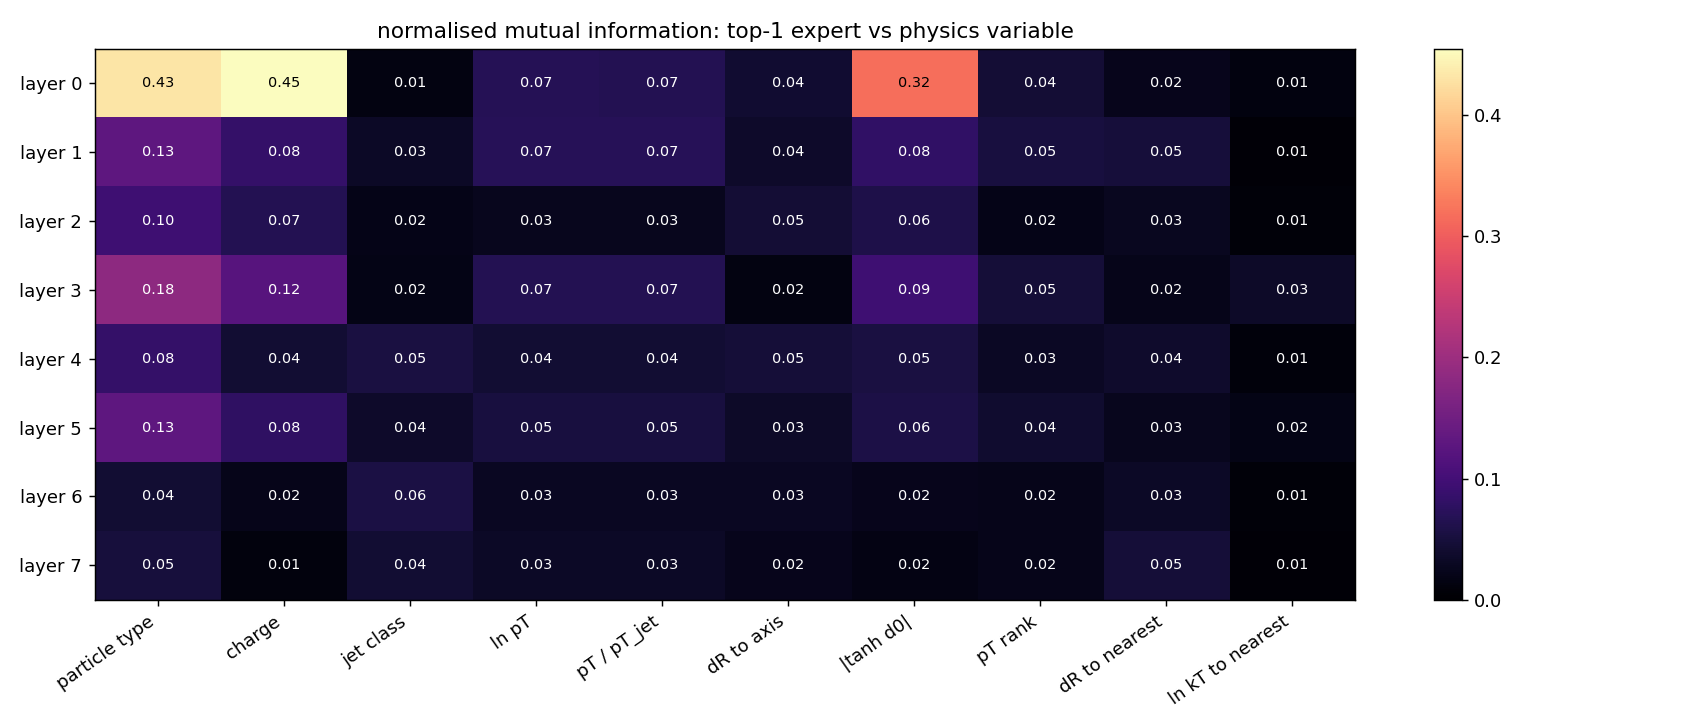
\includegraphics[width=\linewidth]{images/mutual_information.png}
\caption{Normalised mutual information between the top-1 expert and each variable, per layer
(\code{analysis/moe8_short/mutual_information.png}).}
\label{fig:mi}
\end{figure}

Two features stand out (Table~\ref{tab:nmi}, Figure~\ref{fig:mi}):

\begin{enumerate}
 \item \textbf{Layer 0 partitions particles by charge and species.} The NMI with charge is
   0.45 and with particle type 0.43, with $|\tanh d_0|$ at 0.32. Kinematic variables are
   below 0.07. The first router therefore mostly reads particle identity and track
   displacement, which are explicit input features.
 \item \textbf{Deeper layers are nearly uniform.} Router entropy is 2.072--2.075 nats in
   every layer, essentially the maximum of 2.079. Outside layer 0 the largest NMI is 0.18
   (particle type in layer 3), and in layers 4, 6 and 7 no value exceeds 0.09.
   In layers 6 and 7, jet class and nearest-neighbour distance are as informative as type,
   but all values are small.
\end{enumerate}

Loads are balanced: in every layer each expert receives between 8.2\,\% and 17.3\,\% of
top-1 assignments.

\subsection{Layer-0 experts}

\begin{table}[ht]
\centering
\small
\begin{tabular}{@{}crlrrrrr@{}}
\toprule
Expert & Load & Most enriched type & Charged & $\overline{\ln p_T}$ & $\overline{|\tanh d_0|}$ & $\overline{\Delta R}$ & $\overline{\text{rank}}$\\
\midrule
0 & 13.4\,\% & ch.\ had ($1.8\times$) & 0.86 & 1.75 & 0.024 & 0.22 & 23.5\\
1 & 11.9\,\% & muon ($4.5\times$) & 0.89 & 2.02 & \textbf{0.370} & 0.26 & 20.2\\
2 & 12.9\,\% & photon ($2.2\times$) & 0.00 & 1.27 & 0.000 & 0.35 & 28.9\\
3 & 13.0\,\% & ch.\ had ($2.0\times$) & 0.98 & 2.65 & 0.017 & 0.24 & 15.1\\
4 & 13.1\,\% & neu.\ had ($3.3\times$) & 0.56 & 2.07 & 0.013 & 0.18 & 19.1\\
5 & 14.4\,\% & electron ($2.5\times$) & 0.37 & 1.77 & 0.012 & 0.27 & 25.8\\
6 & 11.3\,\% & photon ($2.2\times$) & 0.08 & 1.35 & 0.002 & 0.14 & 27.9\\
7 & 10.0\,\% & neu.\ had ($2.0\times$) & 0.03 & 2.44 & 0.012 & 0.16 & 14.4\\
\bottomrule
\end{tabular}
\caption{Layer-0 expert profiles from \code{report.json}: top-1 load, the particle type with
the largest enrichment $P(e\mid\tau)/\text{load}_e$, charged fraction, and mean
$\ln p_T$, $|\tanh d_0|$, $\Delta R$ to the jet axis and $p_T$ rank of the particles routed
to the expert.}
\label{tab:layer0}
\end{table}

\begin{figure}[ht]
\centering
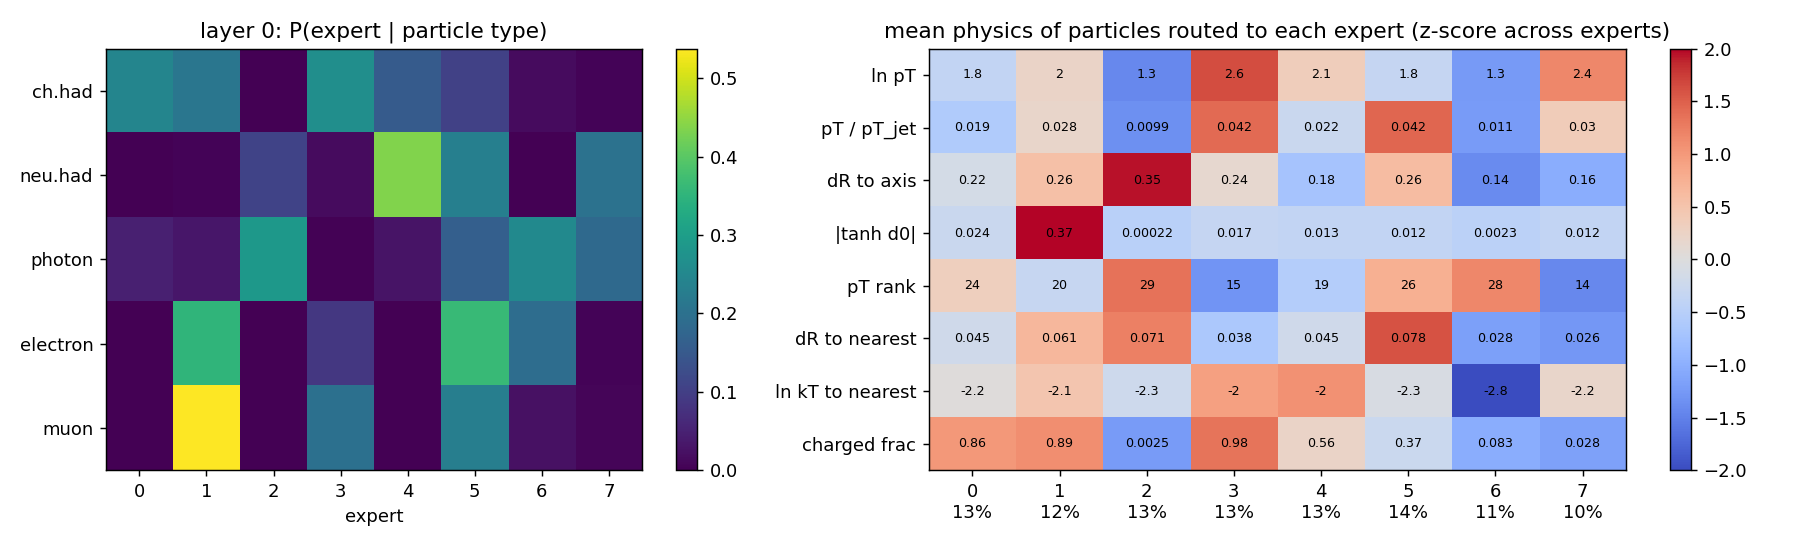
\includegraphics[width=\linewidth]{images/routing_layer0.png}
\caption{Layer 0: $P(\text{expert}\mid\text{particle type})$ (left) and the mean physics of
the particles routed to each expert, as a z-score across experts (right).}
\label{fig:layer0}
\end{figure}

Table~\ref{tab:layer0} and Figure~\ref{fig:layer0} give a readable picture of the first
layer. Experts 2 and 6 take photons: expert 2 the softest, widest-angle ones (mean
$\ln p_T=1.27$, $\Delta R=0.35$), expert 6 photons closer to the axis with small
nearest-neighbour $k_T$, consistent with collinear photon pairs. Experts 4 and 7 are
neutral-hadron experts, and expert 3 takes the hardest charged hadrons (mean rank 15,
$\ln p_T=2.65$). Expert 1 is the clearest case: it is $4.5\times$ enriched in muons, its
particles have by far the largest mean $|\tanh d_0|$ (0.37, against at most 0.024 for the
others), and 53.8\,\% of all muons go to it. It is also the expert most used by Hbb jets:
$P(e=1\mid\text{Hbb})=0.237$ against $0.075$ for QCD. Displaced tracks and soft muons are
the textbook signatures of $b$-hadron decays, so this is the physically expected expert,
found without supervision. Its usage is also high in Tbl jets ($0.205$), which contain a
$b$ quark and a lepton.

\begin{figure}[ht]
\centering
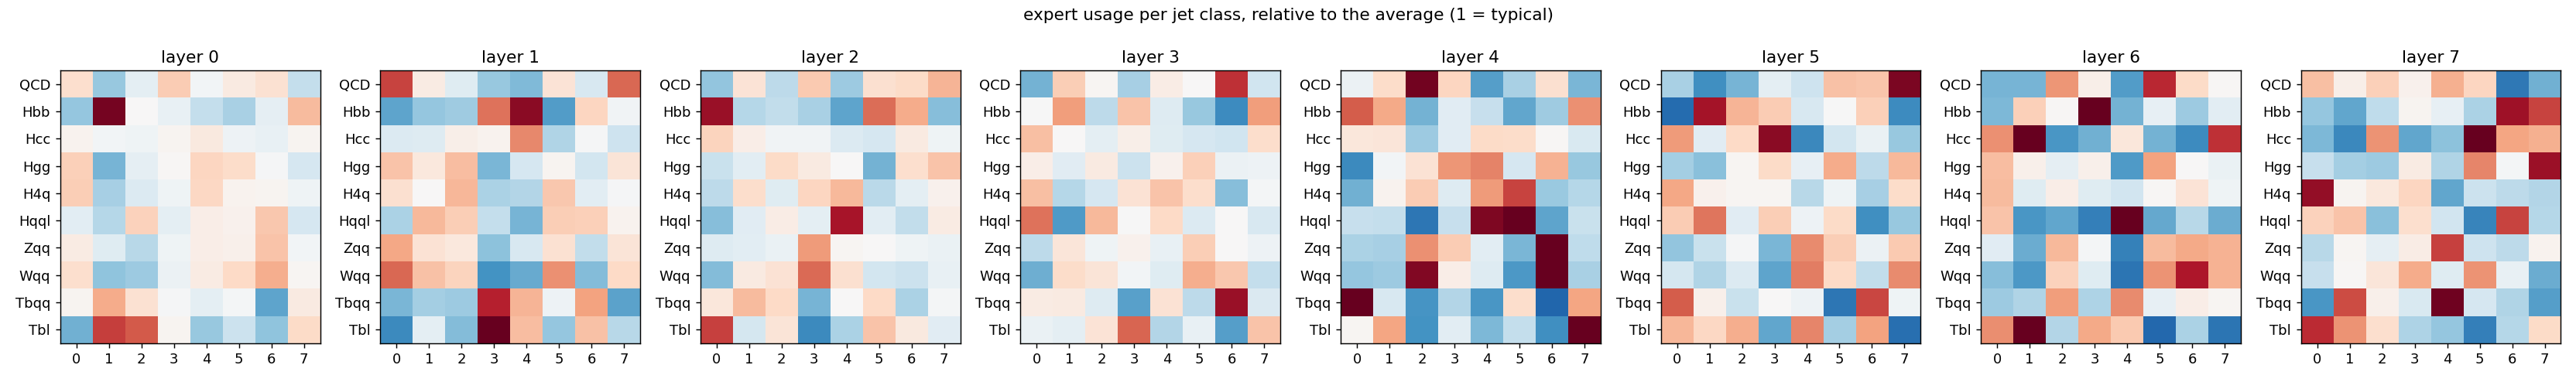
\includegraphics[width=\linewidth]{images/class_usage.png}
\caption{Expert usage per jet class, relative to the average usage, for all eight layers.}
\label{fig:class}
\end{figure}

\subsection{Knockout}
The knockout results in \code{report.json} contain base accuracies for three classes only
(QCD 0.764, Hbb 0.916, Hcc 0.842): the knockout pass used 5{,}000 jets taken in cache order,
which covers only these classes. All changes lie between $-0.2$ and $+0.2$ percentage
points. The changes are multiples of $1/2048$, $1/1955$ and $1/997$ for the three classes,
so each step is a single jet; for example, removing layer-0 expert 3 costs Hcc
$0.2$\,pp, i.e.\ two jets. These effects are within statistical noise. With two experts
per particle and near-uniform routers, the remaining experts (which are still close copies of
the same dense FFN) can absorb the rerouted particles.

\begin{figure}[ht]
\centering
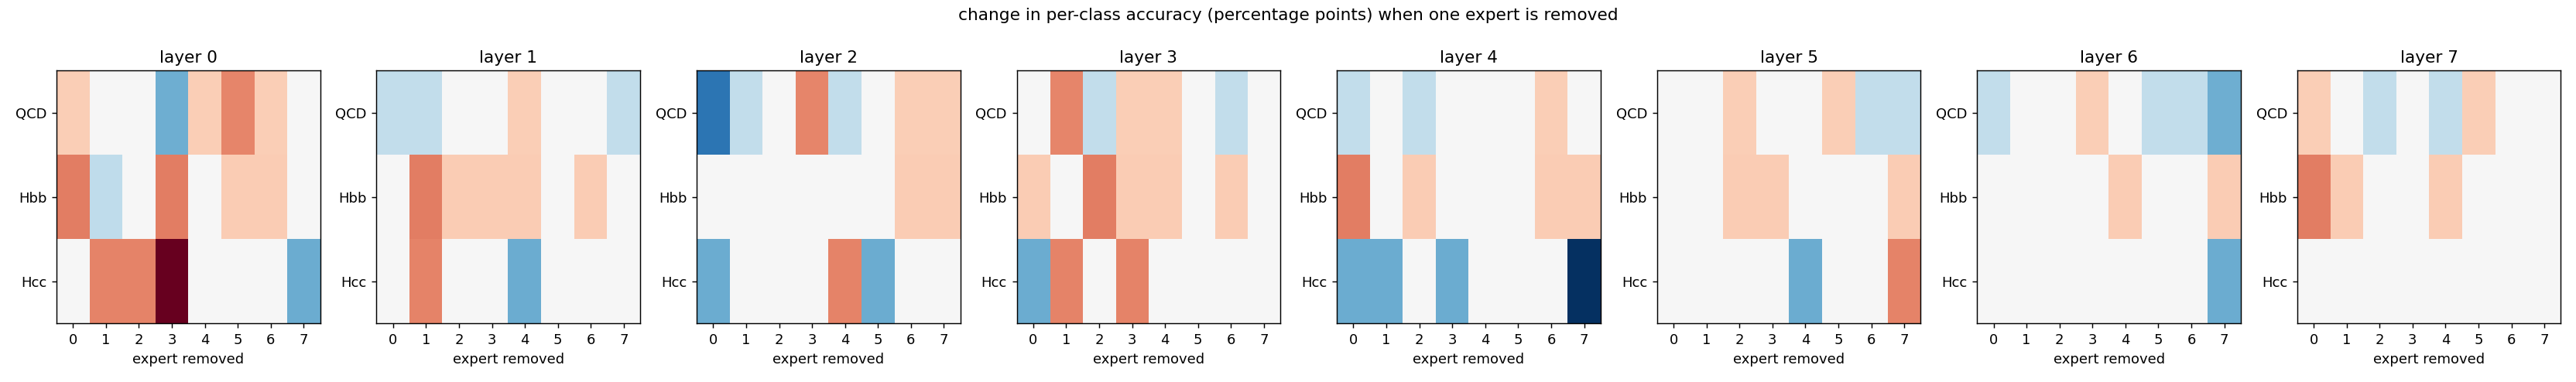
\includegraphics[width=\linewidth]{images/knockout.png}
\caption{Change in per-class accuracy (percentage points) when one expert is removed.}
\label{fig:knockout}
\end{figure}

%====================================================================
\section{Testing}
%====================================================================

\code{tests/test_moe.py} runs on the CPU in a few seconds with a small model ($D=32$, four
heads, three layers, $D_{\rm ff}=64$, four experts, top-2, no dropout) and synthetic jets:

\begin{itemize}
 \item \code{test_upcycle_matches_dense}: an upcycled MoE with $\sigma=0$ reproduces the
   dense logits to $10^{-5}$.
 \item \code{test_padding_and_aux}: changing padded features does not change the output;
   recorded routing covers exactly the real particles; \code{moe_layers=[1,2]} creates MoE
   only there; the auxiliary loss is positive.
 \item \code{test_train_step_and_knockout}: one AdamW step gives every router a non-zero
   gradient; disabled experts are never selected.
\end{itemize}

%====================================================================
\section{Limitations}
%====================================================================

\begin{itemize}
 \item \textbf{Very short fine-tune.} One epoch on 300k jets is far from convergence of the
   expert split. The near-maximal router entropy in layers 1--7 shows that the upcycled
   experts have not yet diverged; conclusions about deeper-layer physics are premature.
 \item \textbf{One seed.} Expert indices are arbitrary and the partition may change with the
   seed. No second run exists yet.
 \item \textbf{Correlation, not mechanism.} NMI and enrichment are correlations. Particle
   type, charge and $d_0$ are direct inputs, so a layer-0 split along them is the easiest
   thing for a linear router to learn. Kinematic variables are themselves correlated with
   species.
 \item \textbf{Top-1 summaries of top-2 routing.} The statistics use only the top-1 expert,
   while the model mixes two experts; a near-uniform $\pi$ can still yield structured top-1
   labels.
 \item \textbf{Small knockout sample.} The stored knockout covers three classes and changes
   of one or two jets. It cannot yet separate real dependence from noise.
 \item \textbf{Auxiliary-loss scaling.} Balance and $z$ losses are summed over layers and
   computed per micro-batch, so their effective strength depends on the number of MoE layers
   and on the micro-batch size.
 \item \textbf{No efficiency gain claimed.} The experts are evaluated in a Python loop with
   gather/scatter; the implementation targets interpretability, not throughput.
\end{itemize}

%====================================================================
\section{Outlook}
%====================================================================

\begin{itemize}
 \item Fine-tune for three or more epochs on the full 10M-jet cache, so that the deeper
   experts have a chance to specialise.
 \item Sweep \code{--aux_weight} $10^{-3}$, \code{--top_k 1} and \code{--moe_layers 4,5,6,7}
   to obtain sharper, easier-to-read routing (keeping in mind the router-gradient caveat of
   top-1).
 \item Repeat with a second seed and compare partitions up to permutation of expert indices.
 \item Run knockout on a class-balanced sample of all ten classes with enough jets for
   statistically meaningful per-class changes.
 \item Upcycle the 20-epoch dense checkpoint once it is available, to start from the strongest
   dense model.
 \item Look for a depth trend in which routing moves from raw inputs (type, charge) in early
   layers to jet-substructure roles (Lund-plane region, class) later. A knockout that mainly
   hurts Hbb/Hcc for an expert with large $|d_0|$ would identify a heavy-flavour expert; one
   that hurts Tbl/Hqql and is lepton-enriched would identify a lepton expert.
\end{itemize}

%====================================================================
\section*{Source map}
%====================================================================
\addcontentsline{toc}{section}{Source map}

\begin{tabularx}{\linewidth}{@{}lX@{}}
\toprule
File & Contents\\
\midrule
\code{moe.py} & \code{GDSParTMoEConfig}, \code{MoEFFN}, \code{GDSParTMoEBlock}, \code{GDSParTMoE},
  \code{upcycle_state_dict}\\
\code{train_moe.py} & data loading, two-group AdamW, warm-up and cosine schedule, AMP,
  micro-batching, evaluation and checkpoints\\
\code{metrics.py} & accuracy, macro OvO AUC, background rejection at fixed signal efficiency\\
\code{analyze_experts.py} & routing recording, physics variables, profiles, NMI, knockout,
  plots and \code{REPORT.md}\\
\code{gds_part_colab.py} & the unchanged GDS-ParT modules\\
\code{data/jetclass_cache.py} & JetClass cache, loader and GPU pair features\\
\code{tests/test_moe.py} & CPU unit tests\\
\code{analysis/moe8_short/} & the analysis of the first run\\
\bottomrule
\end{tabularx}

\end{document}
